\section{A Technical Tool to Quantify the Bias-Variance Trade-off}
\label{sec_main}

%We revisit the classical bias-variance trade-off in the context of multi-task learning for linear regressions, in particular the setup of equation \eqref{eq_mtl}.
We develop a technical tool to derive $\te(\hat{\beta}_t^{\MTL})$ that only depends on the qualities of task data such as data sizes and covariance matrices, for two tasks with general covariances.
Then, we extend the result to more than two tasks that share the same features but have different labels.
Finally, we show a sharp bias-variance tradeoff for transfer learning settings.
%For the high-dimensional setting where the data size of the target task is a small constant times dimension $p$, we quantify the trade-off as a function of the task models $\set{\beta_i}_{i=1}^t$, data size $\set{n_i}_{i=1}^t$, and covariance matrices $\set{\Sigma_i}_{i=1}^t$.

\textbf{Multi-task learning.} applies to the setting of two tasks where their covariance matrices may be arbitrarily different.
%The technical crux of our approach is to derive the asymptotic limit of $\te(\hat{\beta}_t^{\MTL})$ in the high-dimensional setting, when $p$ approaches infinity.
We derive a precise limit of $\bigtr{(X_1^{\top}X_1 + X_2^{\top}X_2)^{-1}\Sigma_2}$, which is a deterministic function that only depends on $\Sigma_1, \Sigma_2$ and $n_1/p, n_2/p$ (see Lemma \ref{lem_cov_shift} in Appendix \ref{app_proof_main} for the result).
Based on the result, we show how to determine positive versus negative transfer as follows.

\begin{theorem}[Informal]\label{thm_main_informal}
	Let $X_i \in\real^{n_i \times p}$ and $Y_i = X_i\beta_i + \varepsilon_i$, for $i = 1, 2$.
	Suppose that $n_1 = \rho_1 p$ and $n_2 = \rho_2 p$, where $\rho_1>1$ and $\rho_2 >1$ are fixed constants.
	There exists two deterministic functions $\Delta_{\beta}$ and $\Delta_{\vari}$ and a small deterministic error $\delta$ that only depend on $\set{\hat{v}, \Sigma_1^{}, n_1, n_2, \beta_1, \beta_2}$ such that
	\begin{itemize}
		\item If $\Delta_{\vari} - \Delta_{\beta} \ge \delta$, then whp $\te(\hat{\beta}_t^{\MTL}) < \te(\hat{\beta}_t^{\STL})$.
		\item If $\Delta_{\vari} - \Delta_{\beta} \le \delta$, then whp $\te(\hat{\beta}_t^{\MTL}) > \te(\hat{\beta}_t^{\STL})$.
	\end{itemize}
\end{theorem}

Theorem \ref{thm_main_informal} shows nearly tight bounds on the trade-off between model-shift bias and variance reduction.
%determined by the covariate shift matrix and the model shift.
The bounds get tighter and tighter as $\rho_1$ increases.
While the general form of $\Delta_{\vari}$ and $\Delta_{\beta}$ can be quite complex, we will show that they provide nice interpretation for simplified settings later on in Section \ref{sec_insight}.

We describe an overview of the proof of Theorem \ref{thm_main_informal}.
By comparing the bias and variance of $\te_t(\hat{\beta}_t^{\MTL})$ to $\te_t(\hat{\beta}_t^{\STL})$, we observe the following two effects, respectively.
%We begin by observing that the test error of $\hat{\beta}_t^{\MTL}$ consists of two parts.
We term equation \eqref{eq_te_model_shift} as \textit{model-shift bias}, which captures how similar $\beta_1$ and $\beta_2$ are.
This part introduces a negative effect to multi-task learning.
The scaling term $\hat{v}$ corresponds to the intuition that the shared module $B$ learns a subspace for both tasks.
The output layer of each task scales the direction of $B$ suitably to fit the task.

Next, it is not hard to verify that equation \eqref{eq_te_var}, the variance of $\hat{\beta}_t^{\MTL}$, is always smaller than the variance of $\hat{\beta}_t^{\STL}$.
This part introduces a positive variance reduction effect to performing multi-task learning.
Hence, whether $\te(\hat{\beta}_t^{\MTL})$ is lower than $\te(\hat{\beta}_t^{\STL})$ is determined by the trade-off between two effects:
(i) the positive effect from variance reduction;
(ii) the negative effect from model shift bias.
A formal version of Theorem \ref{thm_main_informal} is presented in Theorem \ref{thm_model_shift} and its proof is presented in Appendix \ref{app_proof_main}.

\textbf{Extension.} The above result also applies to the setting of more than two tasks with the same covariates.
%We extend the above result to any number of tasks that have the same covariates.
%In this section we consider the setting with $k$ many that have the same covariates.
Since the tasks all have the same number of datapoints and covariance matrix, the trade-off between model shift bias and variance will be captured by their task models $\set{\beta_i}_{i=1}^k$.
%For this setting, we derive solutions for the multi-task training and the transfer learning setting that match our insights qualitatively from Section \ref{sec_denoise}.
%Let $B^{\star} = [\beta_1, \beta_2, \dots, \beta_k] \in\real^{p\times k}$ denote the underlying task model parameters.
We derive a similar trade-off between model shift bias and variance reduction for this setting as well.
The formal statement is stated in Theorem \ref{thm_many_tasks} and its proof can be found in Appendix \ref{app_proof_many_tasks}.

\textbf{Transfer learning.}
We extend the intuition behind Theorem \ref{thm_main_informal} to transfer learning settings.
We provide an analysis of the transfer function of Taskonomy \cite{ZSSGM18} using our setup.
Specifically, the source task encoder consists of the representations learnt from one or more source tasks.
The transfer function then tries to fit the target task data to the source task encoder.
For more details, we refer the reader to Figure 4 in Taskonomy.

We map the procedure to our setup as follows.
First, we obtain the single-task estimator $\hat{\beta}_i$ from the source tasks, for $1\le i \le t-1$.
This forms the shared representation $B = [\hat{\beta}_1,\hat{\beta}_2,\dots,\hat{\beta}_{t-1}]$.
Then, we learn the output layer $W_t$ on the target task by minimizing the following objective
\begin{align}
	g(W_t) = \bignorm{X_t B W_t - Y_t}^2.
\end{align}
After solving $W_t$, we use $\hat{\beta}_t^{\TL} = B W_t$ as the estimator for the target task.
By comparing $\te(\hat{\beta}_t^{\TL})$ to $\te(\hat{\beta}_t^{\STL})$, we observe a similar trade-off between model-shift bias and variance reduction for this setting.
%We use our tools to compare $\te(B W_t)$ to $\te(\beta_t^{\STL})$.
The formal statement is presented in Theorem \ref{prop_taskonomy} and its proof in Appendix \ref{app_proof_sec4}.





\section{Theoretical Implications}
\label{sec_insight}

Based on Theorem \ref{thm_main_informal}, we provide precise interpretations of many empirical phenomena in multi-task learning.
In Section \ref{sec_similarity}, we explain three contributing causes of negative transfer, including model dissimilarity, large source data size and covariate shift.
In Section \ref{sec_benefit}, we describe two implications for positive transfer, including labeled data efficiency and de-noising.

\subsection{Contributing Causes of Negative Transfer}\label{sec_similarity}

It is well-known since the seminal work of Caruana \cite{C97} that how well multi-task learning performs depends on task relatedness.
As a warmup, we first describe an example that rigorously formalizes the connection using our setup.

\textit{The isotropic model.}
	Consider two tasks with isotropic covariances $\Sigma_1 = \Sigma_2 = \id$.
	Recall that each task has data size $n_i = \rho_i \cdot p$, for $i = 1, 2$.
	And $X_1\in\real^{n_1\times p}, X_2\in\real^{n_2\times p}$ denotes the covariates of the two tasks, respectively.
	We assume that for the target task, $\beta_2$ has i.i.d. entries with mean zero and variance $\kappa^2$.
	For the source task, $\beta_1 $ equals $\beta_2$ plus i.i.d. entries with mean $0$ and variance $d^2$.
	The labels are given by $Y_i = X_i\beta_i + \varepsilon_i$, where $\e_i$ consists of i.i.d. entries with mean zero and variance $\sigma_i^2$, for $i=1,2$.
	\footnote{For simplicity, we assume that all the random variables have subexponential decay, while keeping in mind that our results can be applied under weaker moments assumptions as shown in the supplementary material.}

\textbf{Cause 1.}
We measure model dissimilarity as $\norm{\beta_1 - \beta_2}^2$, which is the distance between source and target in the isotropic model.
We derive a sharp threshold when positive transfer transitions to negative transfer, as model dissimilarity increases.
%Based on Theorem \ref{thm_model_shift}, we derive the transition threshold in the following proposition.
Define the following function
\begin{align*}
	\Phi(\rho_1, \rho_2) = \frac{(\rho_1 + \rho_2 - 1)^2}{\rho_1 (\rho_1 + \rho_2) (\rho_2 - 1)}.
\end{align*}

\begin{proposition}[Model dissimilarity]\label{prop_dist_transition}
	In the isotropic model, assume that $\rho_1 > 40$ is a fixed constant.
	Let $\sigma_1 = \sigma_2 = \sigma$.
	Whether $\te(\hat{\beta}_t^{\MTL})$ is lower than $\te(\hat{\beta}_t^{\STL})$ is determined by the ratio between model dissimilarity and $\Phi(\rho_1, \rho_2)$:
	\begin{itemize}
		\item If ${p d^2} < \frac{1}{2}  {\sigma^2}  \cdot \Phi(\rho_1, \rho_2)$, then whp we have that $\te(\hat{\beta}_t^{\MTL}) < \te(\hat{\beta}_t^{\STL})$.
		\item If ${p d^2} \ge 2 {\sigma^2} \cdot \Phi(\rho_1, \rho_2)$, then whp we have that $\te(\hat{\beta}_t^{\MTL}) \ge \te(\hat{\beta}_t^{\STL})$.
	\end{itemize}
\end{proposition}

Proposition \ref{prop_dist_transition} simplifies Theorem \ref{thm_main_informal} in the isotropic model, allowing for a more explicit statement of the bias-variance tradeoff.
We remark that the constants $1/2$ and $2$ in the statement above are chosen for ease of presentation.
In general we can close their gap by increasing $\rho_1$.

\todo{} We illustrate the example with a simulation.
We consider a setting where $p = 200$, $n_1 = 90p$, $n_2 = 30p$.
We fix the target task and vary the source task, in particular the parameter $d$ which determines $\norm{\beta_1 - \beta_2}$.
Figure \ref{fig_model_shift} shows the result.
We observe that Proposition \ref{prop_dist_transition} explains most of the observations in Figure \ref{fig_model_shift}.
%in this proposition (and the following ones) can be replaced with $(1+c_1^{-1/2})^{-4}$ and $(1-c_1^{-1/2})^{-4}$. In particular, these bounds becomes tighter as $c_1$ increases.

The proof of Proposition \ref{prop_dist_transition} involves two parts.
First, in equation \eqref{eq_te_var}, the positive variance reduction effect scales with $n_1 = \rho_1 p$, the number of source task data points.
Second, we show that the negative effect of model-shift bias scales with $pd^2$, which is the expectation of $\norm{\beta_1 - \beta_2}^2$.
The proof, which is based on Theorem \ref{thm_main_informal}, can be found in Appendix \ref{app_proof_31}. %, which is based on our main result described later in Theorem \ref{thm_model_shift}.

\begin{figure}
	\begin{subfigure}[b]{0.32\textwidth}
		\centering
		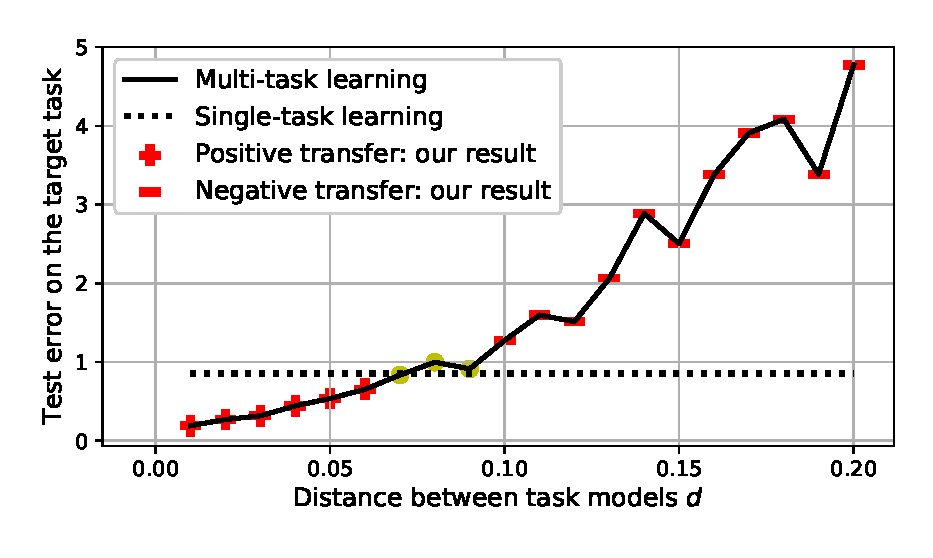
\includegraphics[width=0.98\textwidth]{figures/model_shift_phase_transition.eps}
		\caption{Model dissimilarity}
		\label{fig_model_shift}
	\end{subfigure}\hfill
	\begin{subfigure}[b]{0.32\textwidth}
		\centering
		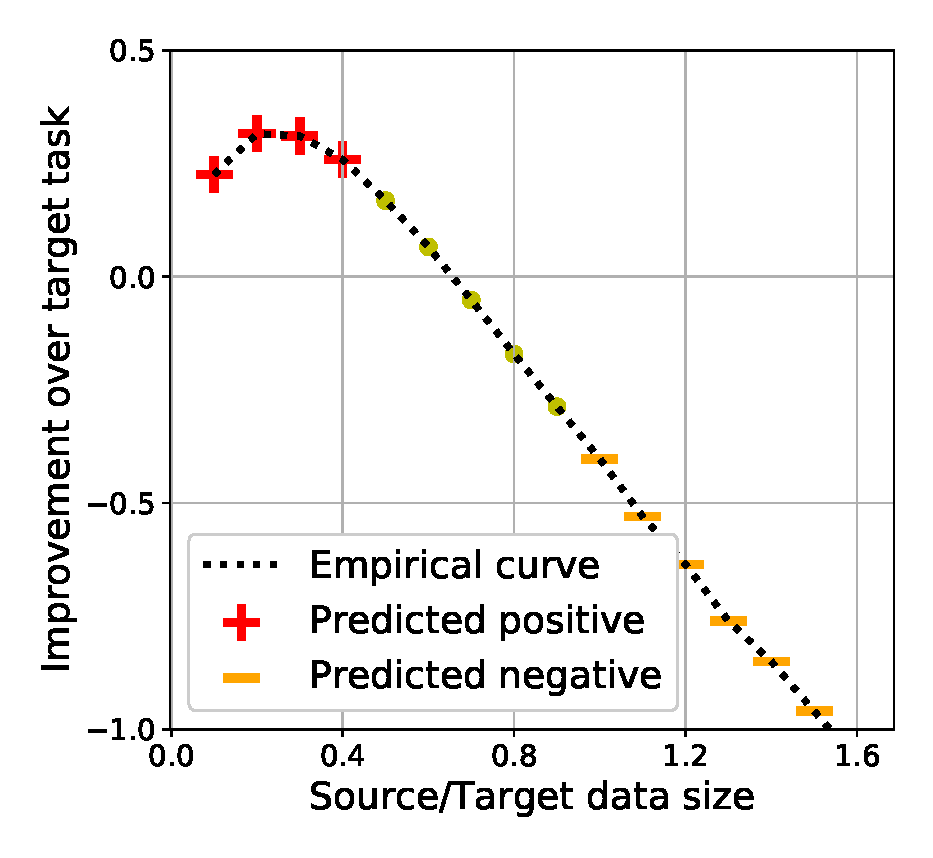
\includegraphics[width=0.98\textwidth]{figures/datapoints_phase_transition.eps}
		\caption{Large source task data size}
	\end{subfigure}\hfill
	\begin{subfigure}[b]{0.32\textwidth}
		\centering
		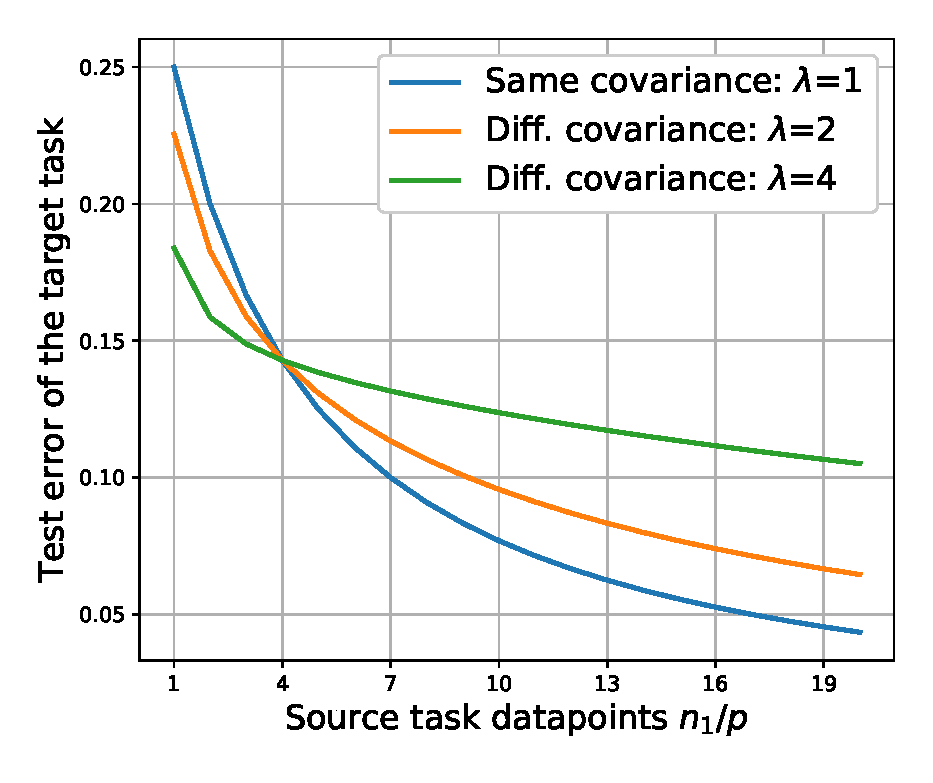
\includegraphics[width=0.98\textwidth]{figures/complementary.eps}
		\caption{Covariate shift}
		\label{fig_covariate}
	\end{subfigure}
	\caption{Three contributing causes of negative transfer:
	(a) As model dissimilarity increases, we observe a transition from positive to negative transfer  (Proposition \ref{prop_dist_transition}).
	(b) As source task data size increases, we observe a transition positive to negative transfer (Proposition \ref{prop_data_size}).
	(c) As covariate shift becomes more severe (measured by increasing $\lambda$), test performance gets worse (Proposition \ref{prop_covariate}).}
	\label{fig_model_shift_phasetrans}
\end{figure}

\textbf{Cause 2.}
In classical Rademacher or VC based theory of multi-task learning, the generalization bounds are usually presented for settings where the data sizes are equal for all tasks \cite{B00,M06,MPR16}.
More generally, such results are still applicable when all task data are being added simultaneously.
On the other hand, for many applications of multi-task learning, the data sources are usually heterogeneous.
For such settings, we have observed that adding more labeled data from one task does not always help.
%On the other hand, we have observed that adding more labeled data does not always improve performance in multi-task learning.
Using the isotropic model, we consider what happens if we vary the source task data size.

\begin{proposition}[Source data size]\label{prop_data_size}
	In the isotropic model, assume that $\rho_1 > 40$ and $\rho_2 > 500$ are fixed constants.
	We have the following conditions to determine whether $\te(\hat{\beta}_t^{\MTL})$ is lower than $\te(\hat{\beta}_t^{\STL})$:
	\begin{itemize}
		\item[a)] If $pd^2 \le \frac{1}{2}\cdot \frac{\sigma^2}{\rho_2-1}$, then whp $\te(\hat{\beta}_t^{\MTL}) < \te(\hat{\beta}_t^{\STL})$ for any $\rho_1 > 40$.
		\item[b)] If $pd^2 > 2\cdot\frac{\sigma^2}{\rho_2 - 1}$, then we have the following transition depending on $\rho_1$:
		\begin{itemize}
			\item If $\rho_1 \cdot p < \frac{(\rho_2-2)\sigma^2}{(1 + {\rho_1}^{-0.5})^4(\rho_2 - 1) d^2 - \sigma^2 / p}$, then whp $\te(\hat{\beta}_t^{\MTL}) < \te(\hat{\beta}_t^{\STL})$.
			\item If $\rho_1 \cdot p > \frac{(\rho_2-2) \sigma^2}{(1 - {\rho_1}^{-0.5})^4 (\rho_2 - 3) d^2 - \sigma^2 / p}$, then whp $\te(\hat{\beta}_t^{\MTL}) > \te(\hat{\beta}_t^{\STL})$.
		\end{itemize}
	\end{itemize}
\end{proposition}
The intuition behind Proposition \ref{prop_data_size} is as follows.
a) If $\norm{\beta_1 - \beta_2}^2 \approx pd^2$ is sufficiently small, then adding any amount of labeled data from the source task always provides positive transfer;
ii) Otherwise, as source data size increases, we observe a transition from positive to negative transfer.
The proof of Proposition \ref{prop_data_size} is similar to Proposition \ref{prop_dist_transition}, and can be found in Appendix \ref{app_proof_31}.

\textbf{Cause 3.}
So far we have considered the isotropic model where $\Sigma_1 = \Sigma_2$.
This setting is relevant for settings where different tasks share the same input features such as multi-class image classification.
In general, the covariance matrices of the two tasks may be different such as in text classification.
In this part, we consider what happens when $\Sigma_1 \neq \Sigma_2$.

We measure covariate shift by the matrix $M = \Sigma_1^{1/2} \Sigma_2^{-1/2}$.
We ask: is it better to have $M$ as being close to identity, or should $M$ involve varying levels of singular values?
Understanding this question has implications for applying normalization methods in multi-task learning \cite{LV19,CBLR18,YKGLHF20}.
We show that if $n_1$ is much larger than $n_2$, then the optimal $M$ matrix should be proportional to identity, under certain assumptions on its range of singular values (to be formulated in Proposition \ref{prop_covariate}).
On the other hand, if $n_1$ is comparable or even smaller than $n_2$, we show an example where having ``complementary'' covariance matrices is better performing than having the same covariance matrices.

	To compare different choices of $M$ on the performance of $\hat{\beta}_t^{\MTL}$, consider the following family of matrices
	\begin{align*}
		\cS_{\mu}\define\bigset{M \mid \det\bigbrace{ M^\top M} \le \mu^p, \lambda(M) \in [\mu_{\min}, \mu_{\max}]},
	\end{align*}
	where $\mu, \mu_{\min}, \mu_{\max}$ are fixed values that do not grow with $p$. We first assume that there is no model bias. 
	Similar to the isotropic model, we assume that $\beta_1=\beta_2$ has i.i.d. entries with mean zero and variance $\kappa^2$.
	The following proposition shows that when $n_1$ is much larger than $n_2$, $\te(\hat{\beta}^{\MTL})$ is minimized at $M = \mu\id$ among all matrices in $\cS_{\mu}$.

\begin{proposition}[Covariate shift]\label{prop_covariate}
	In the setting described above, assume that $\rho_1 > 1$ and $\rho_2>1$.
	Let $g(M)$ denote the test error of $\hat{\beta}_t^{\MTL}$ when the covariance shift matrix is equal to $M\in\cS_{\mu}$.
	We have that \[ g(\mu\id) \le \bigbrace{1+ \bigo{\frac{\rho_2}{\rho_1}  }} \min_{M\in\cS_{\mu}} g(M). \]
\end{proposition}
Proposition \ref{prop_covariate} implies that when $\rho_1\gg \rho_2$, having no covariate shift is the optimal choice for choosing the source task.
%This provides evidence that covariate shift is unfavorable when there are many source task datapoints,

\todo{} To complement the result, we show an example when the statement is not true if $n_1 \le n_2$.
\begin{example}\label{ex_complement}
	In the setting of Proposition \ref{prop_covariate}, we compare two cases: (i) when $M = \id$; (ii) when $M$ has $p/2$ singular values that are equal to $\lambda$ and $p/2$ singular values that are equal to $1 / \lambda$.
	For simplicity, we assume that $d = 0$.
	Hence the two tasks have the same model parameters.

	In Figure \ref{fig_model_shift_phasetrans} (c), we plot the test error of the target task for $n_2 = 4p$ and $n_1$ ranging from $p$ to $20p$.
	Second, we observe the following two phases as we increase $n_1 / p$.
	When $n_1 \le n_2$, having complementary covariance matrices leads to lower test error compared to the case when $\Sigma_1 = \Sigma_2$.
	When $n_1 > n_2$, having complementary covariance matrices leads to higher test error compared to the case when $\Sigma_1 = \Sigma_2$.
	A theoretical justification can be found in Appendix \ref{app_proof_31}.
\end{example}


\subsection{Implications for Positive Transfer}\label{sec_benefit}

On the positive side, we describe two implications for positive transfer, assuming that $\norm{\beta_1 - \beta_2}^2$ is small in the isotropic model.

\textbf{Implication 1.}
We use our tools to explain a key result of taskonomy \cite{ZSSGM18}, which shows that by learning from multiple related tasks, one can reduce the amount of labeled data from each task.
This is formalized by a metric called the data efficiency ratio as follows.

Given several tasks, let $\alpha^{\star}$ be the largest factors such that the total number of labeled datapoints needed for solving all tasks can be reduced by an $\alpha^{\star}$ factor (compared to training independently) while keeping the same performance.
%More precisely, suppose we have $n_i$ datapoints for each task, for $i= 1, 2$.
For $i = 1, 2$, let $\hat{\beta}_i^{\MTL}(\alpha)$ denote the estimator trained using only $\alpha n_i$ datapoints from every task.
The data efficiency ratio is defined as
\[ \alpha^{\star} \define\argmin_{\alpha\in(0, 1)} ~~
		\te_1(\hat{\beta}_1^{\MTL}(\alpha)) + \te_2(\hat{\beta}_2^{\MTL}(\alpha))
		\le \te_1(\hat{\beta}_1^{\STL}) + \te_2(\hat{\beta}_2^{\STL}). \]
We quantify the data efficiency ratio of the isotropic model as follows.

\begin{proposition}[Labeled data efficiency]\label{prop_data_efficiency}
	In the isotropic model, assume that $\rho_1$ and $\rho_2$, $pd^2 < {8\sigma^2} /{(3 \rho)}$.
	Then the data efficiency ratio is at most $\frac{1}{2\rho} + \frac{\sigma^2}{2\sigma^2 - 3p d^2 \rho / 4}$.
\end{proposition}
The proof of Proposition \ref{prop_data_efficiency} can be found in Appendix \ref{app_proof_data}.

\textbf{Implication 2.}
We further show that multi-task learning is particular powerful when the labeled data of the source task is less noisy compared to the target task.
Consider a more general setting of Proposition \ref{prop_dist_transition} where the noise level $\sigma_1$ of task $1$ differs from the noise level $\sigma_2$ of task $2$.
We extend Proposition \ref{prop_dist_transition} as follows.

\begin{proposition}[Labeled data de-noising]\label{prop_var_transition}
	In the isotropic model, assume that $\rho_1 > 40$ and $pd^2 < \frac{1}{2} {\sigma_2^2}  \cdot \Phi(\rho_1, \rho_2)$.
	We derive the following transition as a parameter of $\sigma_1^2$:
	\begin{itemize}
		\item If $\sigma_1^2 \le -2 \rho_1 \cdot p d^2+\left(1+ \frac34\rho_1 \Phi(\rho_1, \rho_2)\right)\cdot\sigma_2^2$, then whp $\te(\hat{\beta}_t^{\MTL}) < \te(\hat{\beta}_t^{\STL})$.
		\item If $\sigma_1^2 > - \frac12\rho_1\cdot p d^2   +\left(1+ \frac32\rho_1\Phi(\rho_1, \rho_2)\right) \cdot \sigma_2^2$, then whp $\te(\hat{\beta}_t^{\MTL}) > \te(\hat{\beta}_t^{\STL})$.
	\end{itemize}
\end{proposition}
As a corollary, if $\sigma_1^2 \le \sigma_2^2$, then we always get positive transfer.
The proof of Proposition \ref{prop_var_transition} is similar to Proposition \ref{prop_dist_transition}.
The details can be found in Appendix \ref{app_proof_data}.



